\documentclass[american]{scrartcl}

    \newcommand{\lang}{en}

    \usepackage{babel}
    \usepackage[utf8]{inputenc} 
    \usepackage{csquotes}
    \usepackage{amsmath, amssymb}
    \usepackage{graphicx}
    \usepackage{tikz} 
    \usepackage{mathtools}
    \usepackage{bm}

    \setlength{\parindent}{0em}
    \setlength{\parskip}{0.5em}
	\setlength{\fboxsep}{1em}


    % Graphs
    \usetikzlibrary{positioning, arrows.meta, calc, decorations.markings, math, matrix}

    \tikzset{main node/.style={circle, draw,minimum size=2cm,inner sep=3pt},}

    % Math commands
    \newcommand{\E}{\mathbb{E}}
    \newcommand{\R}{\mathbb{R}}

    \newcommand{\matr}[1]{\bm{#1}}
	\newcommand{\set}[1]{\left\{#1\right\}}
	\newcommand{\diag}{\text{diag}}

	\DeclareMathOperator{\Tr}{Tr}

    \DeclarePairedDelimiter\abs{\lvert}{\rvert}%
    \DeclarePairedDelimiter\norm{\lVert}{\rVert}%


    \usepackage[
        bibencoding=utf8, 
        style=apa
    ]{biblatex}

    \bibliography{../../../Desktop/bibliographies/thesis, ../maths}
    
    
    \usepackage{amsmath}
    \title{
        Prosumer Electricity Markets
    }

    \subtitle{Model}

    \author{Andrea Titton}
    
\begin{document}

\nocite{*}
\maketitle

\tableofcontents
\newpage

\section*{Mathematical notation}

\begin{itemize}

	\item Matrices will be represented with bold characters, $\matr{A}$, and graphs with calligraphic characters, $\mathcal{A} = (V, E)$, where $V$ is the set of vertices and $E$ the set of edges.

	\item The operator $\diag$ sets all the off-diagonal entries to zero, \begin{equation*}
		      \diag: \R^{n \times n} \to \R^{n \times n}, \ \ \diag(\matr{A}) = \begin{pmatrix}
			      a_{1, 1} & 0        & \ldots   &                   \\
			      0        & a_{2, 2} & 0        & \ldots &          \\
			      \vdots   & 0        & a_{3, 3} & 0      & \ldots   \\
			               &          & 0        & \ddots &        & \\
		      \end{pmatrix}
	      \end{equation*}

	\item I am using element-wise (Hadamard) operations between vertices and matrices extensively in the grid problem. The notation is the following, \begin{equation}
		      \begin{split}
			      \text{With }x, y &\in \R^n \\
			      x \circ y &= \begin{pmatrix}
				      x_1 \cdot y_1 \\ x_2 \cdot y_2 \\ \vdots \\ x_n \cdot y_n
			      \end{pmatrix}, \ \
			      x \oslash y = \begin{pmatrix}
				      x_1 / y_1 \\ x_2 / y_2 \\ \vdots \\ x_n / y_n
			      \end{pmatrix}, \ \
			      x^{\circ m} = \begin{pmatrix}
				      x_1^m \\ x_2^m \\ \vdots \\ x_n^m
			      \end{pmatrix}
		      \end{split}
	      \end{equation}

\end{itemize}


\section{Network structure}

\begin{minipage}{0.45\textwidth}{
		\resizebox{\textwidth}{!}{
			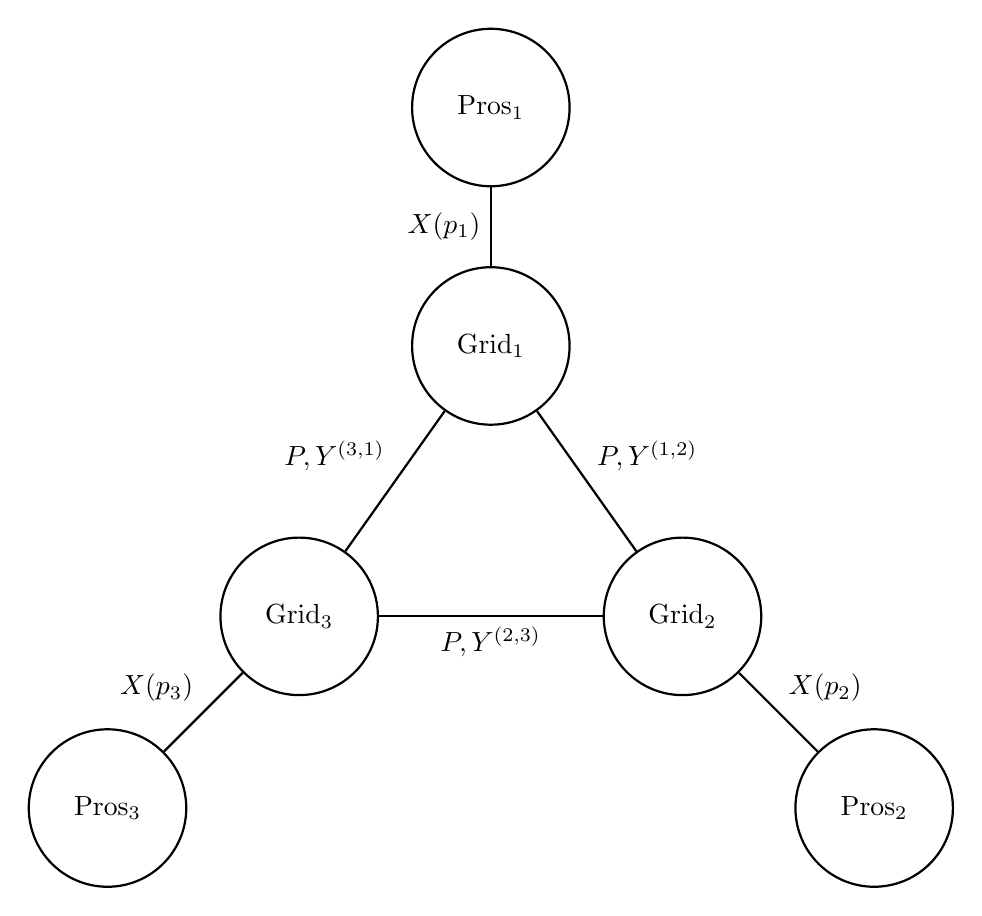
\begin{tikzpicture}[-, thick]
				% Grids
				\node[main node] (1) {Grid$_1$};
				\node[main node] [below right = 2cm and 1cm of 1] (2) {Grid$_2$};
				\node[main node] [below left = 2cm and 1cm of 1] (3) {Grid$_3$};
				% Local markets 
				\node[main node] [above = 1cm of 1] (5) {Pros$_1$};
				\node[main node] [below right = 1cm and 1cm of 2] (6) {Pros$_2$};
				\node[main node] [below left = 1cm and 1cm of 3] (7) {Pros$_3$};
				% Paths
				\path[draw,thick]
				(1) edge node [above right] {$P, Y^{(1, 2)}$} (2)
				(2) edge node [below] {$P, Y^{(2, 3)}$} (3)
				(3) edge node [above left] {$P, Y^{(3, 1)}$} (1)
				(1) edge node [left] {$X(p_{1})$} (5)
				(2) edge node [above right] {$X(p_{2})$} (6)
				(3) edge node [above left] {$X(p_{3})$} (7);
			\end{tikzpicture}
		}}\end{minipage} \hfill
\begin{minipage}{0.5\textwidth}{
		The model is structured on two levels: local prosumer markets ($Pros_i$) and global electricity markets ($Grid_i$). The former are composed of heterogenous agents endowened with electricity and risk averse with respect to electricity consumption. The excess (defect) of energy generates a supply (demand) of electricity which is absorbed (met) by grid firms on the ``global'' energy market. These trade electricity with each other via bilateral bargaining.
	}
\end{minipage}

\section{Prosumers}

\subsection{Log utility}

The prosumer instantaneous utility of electricity consumption is,

\begin{equation*}
	u_i(x) = d \cdot \ln(x),
\end{equation*}

where $d$ is a scale parameter.

Each period, agents are endowed electricity, $e_{i, t}$, which follows a random exogenous process and have a given stock of cash-in-hand $m_{i, t}$. Furthermore agents can buy or sell electricity $x_{i, t}$ at price $p_t$. $x_{i, t} > 0$ implies that agents are buying electricity and $x_{i, t} < 0$ that they are selling it.

Suppressing $i$ for convenience, the dynamic optimization problem is then,

\begin{equation*}
	\begin{split}
		V(e_t) &= \sup_{x_t \in \R} \left\{u(x_t + e_t) + \beta \cdot \E_t V( e_{t+1} ) \right\} \\
		\\
		\textit{s.t. } m_{t+1} &= m_{t} - p_{t} \cdot x_{t}\\
		m_t  &\geq 0
		\\
		\textit{given } m_0&
	\end{split}
\end{equation*}

Agents are assumed to make forecasts over the price $p_{t+1}$, using a linear forecasting rule $\E_t[p_{t+1}] = \psi_h\cdot p_t + c$, where $c$ is a constant and $\psi_h \in \Psi$ is selected in a manner similar to \citeauthor{Hommes2013} (\citeyear{Hommes2013}).

Using the evolution of $m_t$ we can express the individual electricity demanded as,

\begin{equation}
	x_t = \frac{m_t - m_{t+1}}{p_t},
\end{equation}

such that the agents' control variable is the next level of cash-in-hand $m_{t+1}$. This yields the Euler equation,

\begin{equation}
	u^\prime\left( e_t + \frac{m_t - m_{t+1}}{p_t} \right) = \beta \cdot \E_t \left[ u^\prime\left(e_{t+1} + \frac{m_{t+1} - m_{t+2}}{ \psi_h \cdot p_t + c} \right)  \right].
\end{equation}

The endogenous grid method can then be used to numerically find a policy function

\begin{equation}
	m^\prime(m_t \ \vert \ \psi_h, p_t, e_t).
\end{equation}

The solution of the local problem yields the electricity demand given an endowment and different levels of $m_t$. The demand is plotted in Figure \ref{fig:demand}. Furthermore, in Figure \ref{fig:sim} I plot a simulation run of electricity demanded by an agent $x_t$ given an exogenous price mechanism.

\subsection{Discrete aggregation}

Each prosumer market is composed of a discrete number of agents indexed by $i \in \set{1, 2, \ldots n}$. Each period the demand of agent $i$ is,

\begin{equation}
	x_{i, t}(p_t \ \vert \ e_t) = \frac{m_{i, t} - m^\prime(m_{i, t} \ \vert \ \psi_h, p_t, e_t).}{p_t}
\end{equation}

which yields aggregate demand,

\begin{equation}
	X_t(p_t) = \sum^n_{i = 1} x_{i, t}(p_t \ \vert \ e_t)
\end{equation}


\subsection{To do}

I would like the preferences to be Epstein-Zin, but could not find a solution to the problem at hand.

\section{Grid firms}

\subsection{Notation}

Grid firms do not face any intertemporal optimization. Each period they set the price on the local market $p$ and induce a demand (supply) $X(p)$. They then match $X(p)$ by trading with other grid firms quantities $Y$ at a bargained price $P$. Hence, hereafter I will suppress the time index $t$.

Grid firms operate on a graph $\mathcal{A} = (V, E)$. Firms are nodes, $i \in V$, and they can trade if they share an edge, $(i, j) \in E$. I will indicate the neighbors of a node as,

\begin{equation}
	N_{\mathcal{A}}(i) = \set{ \ j \in V: \ (i, j) \in E \ }
\end{equation}

\subsection{Setup}

Each period, the optimization problem of the firm is,

\begin{equation}
	\max_{p, Y} \Pi_i(p, Y)
\end{equation}

where,

\begin{equation}
	\Pi_i\left(p, Y\right) = X_i(p) \cdot p - \sum_{j \in N_{\mathcal{A}}(i)} Y^{(i, j)} \cdot P^{(i, j)}
\end{equation}

subject to,

\begin{equation}
	X_i=  \sum_{j \in N_{\mathcal{A}}(i)} Y^{(i, j)}
\end{equation}

For now assume $P^{(i, j)}$ is determined by (i.e. is a function of) the vector of traded quantities $Y$, with elements $Y^{(i, j)}$ for every $(i, j) \in E$. Suppressing $i$ for convenience (i.e. $Y^{(i, j)} \mapsto Y_j$), the Lagrangian is,

\begin{equation}
	\mathcal{L}\left(p, Y_j\right) = X(p) \cdot p - \sum_{j \in N_{\mathcal{A}}(i)} Y_j \cdot P_j (Y) + \lambda\cdot \left(X(p) - \sum_{j \in N_{\mathcal{A}}(i)} Y_j\right)
\end{equation}

with first order condition,

\begin{equation}
	\begin{split}
		\frac{\partial \mathcal{L}}{\partial p}  &= \frac{\partial X}{\partial p}(p) \cdot p + X(p) + \lambda \cdot \frac{\partial X}{\partial p}(p) = 0 \\
		\frac{\partial \mathcal{L}}{\partial Y^j}  &= P_j + \frac{\partial P_j}{\partial Y_j} \cdot Y_j + \lambda =0, \ \forall j \in N_{\mathcal{A}}(i)
	\end{split}
\end{equation}

Isolating the multiplier $\lambda$ from the first equation yields,

\begin{equation}
	- \lambda = p + \frac{X}{\partial X / \partial p}
\end{equation}

which, substituting in the second one, yields the system of equations, $\forall j \in N_{\mathcal{A}}(i)$,

\begin{equation} \label{firm_optimization}
	P_j(Y_j) + \frac{\partial P_j}{\partial Y_j} \cdot Y_j = p + \frac{X}{\partial X / \partial p}
\end{equation}

\subsection{Bargaining model}

To solve the bargaining model we need to impose a ``direction'' of trade, namely a traded quantity $Y^{(i, j)}$ enters positively in $j$ and negatively in $i$. To do this we can work with the directed graph $\mathcal{A}$ with upper triangular adjacency matrix $\matr{A}_{d}$.

To encode the asymmetry of trade hereafter I will work with the bi-directed graph with adjacency matrix,

\begin{equation}
	\matr{A} := \matr{A}_{d} - \matr{A}_{d}^T,  \ \matr{A} \in\R^{n\times n}.
\end{equation}

This matrix has entries $a_{i, j} \in \set{-1, 0, 1}$ with $a_{i, j} = - a_{j, i}$ and $a_{i, i} = 0$. For example, the graph of Section 1 would then be represented by,

\begin{equation}
	\matr{A}_d= \begin{pmatrix}
		0 & 1 & 1 \\
		0 & 0 & 1 \\
		0 & 0 & 0
	\end{pmatrix} \implies
	\matr{A} = \begin{pmatrix}
		0  & 1  & 1 \\
		-1 & 0  & 1 \\
		-1 & -1 & 0
	\end{pmatrix}
\end{equation}

The payoff of firm $i$ from the bargaining procedure can be written as,

\begin{equation}
	\begin{split}
		\Pi_i &= X_i(p_i)\cdot p_i - \sum_{j \in N_{\mathcal{A}}(i)} Y^{(i, j)} \cdot P^{(i, j)} \\
		&= X_i(p_i)\cdot p_i - \sum_{j \in V} a_{i, j} \cdot Y^{(i, j)} \cdot P^{(i, j)}
	\end{split}
\end{equation}

The Nash bargaining solution is such that,

\begin{equation}
	P^{(i, j)} = \arg \max_{P^{(i, j)}} \left\{\Pi_i \cdot \Pi_j \right\}.
\end{equation}

The first order condition is,

\begin{equation}
	\frac{\partial\Pi_i}{\partial P^{(i, j)}} \cdot \Pi_j + \frac{\partial\Pi_j}{\partial P^{(i, j)}} \cdot \Pi_i = 0.
\end{equation}

using,

\begin{equation}
	\frac{\partial\Pi_i}{\partial P^{(i, j)}} = - a_{i, j} \cdot Y^{(i, j)} = -\frac{\partial \Pi_j}{\partial P^{(i, j)}}
\end{equation}

we can rewrite the first order condition as,

\begin{equation} \label{foc_2}
	\begin{split}
		\Pi_i &= \Pi_j \\
		X_i(p_i)\cdot p_i - \sum_{m \in N} a_{i, m} \cdot Y^{(i, m)} \cdot P^{(i, m)} &= X_j(p_j)\cdot p_j - \sum_{m \in N} a_{j, m} \cdot Y^{(j, m)} \cdot P^{(j, m)}
	\end{split}
\end{equation}

Using $a_{i, j} = - a_{j, i}$, we can rewrite the two sums in (\ref{foc_2}) as,

\begin{equation}
	\begin{split}
		\sum_{m \in N} a_{i, m} \cdot Y^{(i, m)} \cdot P^{(i, m)} &= \sum_{m \in N \setminus \set{j}}  a_{i, m} \cdot Y^{(i, m)} \cdot P^{(i, m)} + a_{i, j} \cdot Y^{(i, j)} \cdot P^{(i, j)} \ \text{ and }\\
		\sum_{m \in N} a_{j, m} \cdot Y^{(j, m)} \cdot P^{(j, m)} &=  \sum_{m \in N \setminus \set{i}}  a_{j, m} \cdot Y^{(j, m)} \cdot P^{(j, m)} - a_{i, j} \cdot Y^{(i, j)} \cdot P^{(i, j)}
	\end{split}
\end{equation}

which yields, for every edge $(i, j)$ with $ a_{i, j} \neq 0$,

\begin{equation} \label{solution}
	\begin{split}
		P^{(i, j)} = \frac{1}{2\cdot Y^{(i, j)}} \Biggl( &\underbrace{X_i(p_i)\cdot p_i - X_j(p_j)\cdot p_j}_{\text{revenue difference }}
		\\  + &\underbrace{\sum_{m\in N\setminus \set{i}} a_{j, m} \cdot Y^{(j, m)} \cdot P^{(j, m)}}_{\text{outside option of } j}
		\\ - & \underbrace{\sum_{m \in N\setminus \set{j}} a_{i, m} \cdot Y^{(i, m)} \cdot P^{(i, m)}}_{\text{outside option of } i} \Biggr).
	\end{split}
\end{equation}

\subsubsection{Line graph and matrix notation}

% FIXME: This is the incidence matrix

To write Equation (\ref{solution}) in matrix notation, I introduce the line graph associated with our original graph. This is useful because all the vectors of interest, $P, Y, \Delta X$, are vectors over edges rather than nodes. A line graph is the graph with adjacency matrix $\matr{G}(\matr{A}) \in \R^{\abs{E} \times \abs{E}}$ were the nodes are edges of the original graphs and edges are inner nodes of the original graph

For example, consider the graph,

\vspace{0.5em}
\begin{minipage}{0.6\textwidth}
	\resizebox{\textwidth}{!}{
		\begin{tikzpicture}[{Latex[scale=1.25]}-{Latex[scale=1.25]}, thick]
			% Grids
			\node[main node] (1) {$1$};
			\node[main node] [right = 2cm of 1] (2) {$2$};
			\node[main node] [below right = 2cm and 2cm of 2] (5) {$5$};
			\node[main node] [above right = 2cm and 2cm of 2] (3) {$3$};
			\node[main node] [right = 2cm of 3] (4) {$4$};
			% Paths
			\path[draw,thick]
			(1) edge node [above] {$(1, 2)$} (2)
			(2) edge node [below left] {$(2, 5)$} (5)
			(2) edge node [above left] {$(2, 3)$} (3)
			(3) edge node [above] {$(3, 4)$} (4);
		\end{tikzpicture}}
\end{minipage} \hfill
\begin{minipage}{0.35\textwidth}
	\begin{equation*}
		\matr{A} = \begin{pmatrix}
			0  & 1  & 0  & 0 & 0 \\
			-1 & 0  & 1  & 0 & 1 \\
			0  & -1 & 0  & 1 & 0 \\
			0  & 0  & -1 & 0 & 0 \\
			0  & -1 & 0  & 0 & 0
		\end{pmatrix}
	\end{equation*}
\end{minipage}


The corresponding line graph is,

\vspace{0.5em}
\begin{minipage}{0.6\textwidth}
	\resizebox{\textwidth}{!}{
		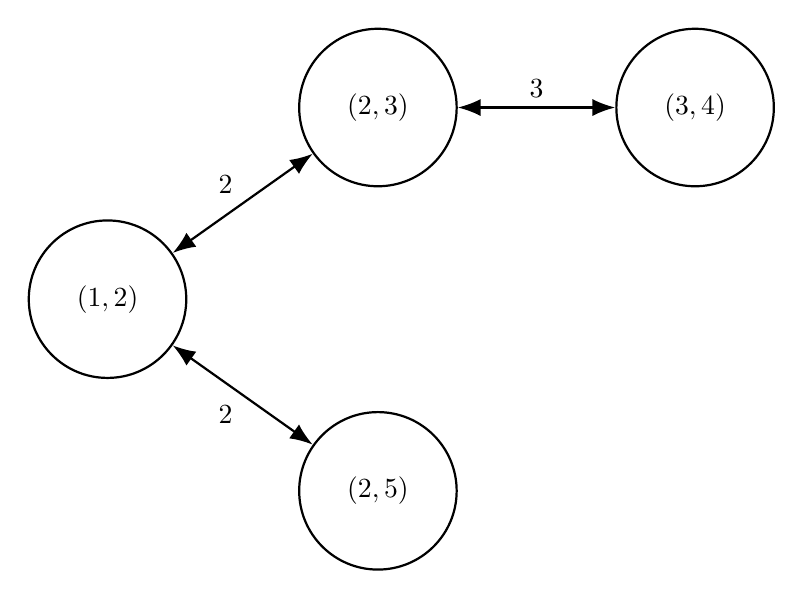
\begin{tikzpicture}[{Latex[scale=1.25]}-{Latex[scale=1.25]}, thick]
			% Grids
			\node[main node] (12) {$(1, 2)$};
			\node[main node] [below right = 1cm and 2cm of 12] (25) {$(2, 5)$};
			\node[main node] [above right = 1cm and 2cm of 12] (23) {$(2, 3)$};
			\node[main node] [right = 2cm of 23] (34) {$(3, 4)$};
			% Paths
			\path[draw,thick]
			(12) edge node [below left] {$2$} (25)
			(12) edge node [above left] {$2$} (23)
			(23) edge node [above] {$3$} (34);
		\end{tikzpicture}}
\end{minipage} \hfill
\begin{minipage}{0.35\textwidth}
	\begin{equation*}
		\matr{G}(\matr{A}) = \begin{pmatrix}
			0   & 1 & 1   & 0 \\
			- 1 & 0 & 0   & 0 \\
			- 1 & 0 & 0   & 1 \\
			0   & 0 & - 1 & 0
		\end{pmatrix}
	\end{equation*}
\end{minipage}




\subsubsection{Line graph and bargaining solution}

In the bargaining problem we have a set of directed edges $E = \set{i \to j: i, j \in N}$. On each edge a bargaining price and a transferred quantity is determined. This defines the two vectors $P, \ Y \in \R^{\abs{E}}$. Furthermore let $\Delta X$ in $\R^{\abs{E}}$ be the vector of revenue difference with entries,

\begin{equation}
	\Delta X^{(i, j)} = X_i(p_i) \cdot p_i - X_{j}(p_j) \cdot p_j
\end{equation}

Equation (\ref{solution}) can be then written as,

\begin{equation} \label{matrix_solution}
	\begin{split}
		2(P \circ Y) &= \Delta X - \matr{G} \left( P \circ Y \right) \\
		(2\matr{I} + \matr{G}) (P \circ Y) &= \Delta X \\
		(P \circ Y) &= (2\matr{I} + \matr{G})^{-1} \Delta X \\
		P &= (2\matr{I} + \matr{G})^{-1} (\Delta X \oslash Y)
	\end{split}
\end{equation}

where $\circ$ and $\oslash$ denote the element-wise (Hadamard) product and division respectively. Using the Neumann expansion of $(2\matr{I} + \matr{G})^{-1}$ (see Appendix \ref{a:neumann}) we obtain,

\begin{equation} \label{neumann_matrix_solution}
	P = \sum^{\infty}_{k=0}\frac{(-1)^k}{2^{k+1}} \matr{G}^k (\Delta X \oslash Y)
\end{equation}

\subsection{Solution of the bargaining problem}

Note that (\ref{neumann_matrix_solution}) defines the bargaining price as a function of the traded quantity $P(Y)$. Let $\partial P$ be the vector of derivatives $\partial P^{(i, j)} / \partial Y^{(i, j)}$ (i.e. the diagonal of the Jacobian, $J_P$).

\begin{equation}
	\partial P = - \diag\left(\sum^\infty_{i=0} \frac{(-1)^k}{2^{k+1}} \matr{G}^k\right) \Delta X \oslash Y^{\circ 2}
\end{equation}

We can use this in equation (\ref{firm_optimization}),

\begin{equation} \label{foc_grid}
	\begin{split}
		P + \partial P \circ Y &= \sum^{\infty}_{k=0}\frac{(-1)^k}{2^{k+1}} \matr{G}^k (\Delta X \oslash Y) - \diag\left(\sum^\infty_{i=0} \frac{(-1)^k}{2^{k+1}} \matr{G}^k\right) (\Delta X \oslash Y^{\circ 2}) \circ Y \\
		&= \underbrace{\left[ \sum^{\infty}_{k=0}\frac{(-1)^k}{2^{k+1}} \matr{G}^k - \diag \left( \sum^{\infty}_{k=0}\frac{(-1)^k}{2^{k+1}} \matr{G}^k \right) \right]}_{\matr{H(G)}} (\Delta X \oslash Y)
	\end{split}
\end{equation}

The matrix $\matr{H(G)}$ is an hollow matrix by construction (i.e. $\matr{H(G)}_{i, i} = 0 \ \forall i$).

\subsection{Equilibrium}

\subsection{To do}

Find a way to link equation $P + \partial P \circ Y$ with the optimization problem of the grid firm. It seems like $(P + \partial P \circ Y)_j = p + \frac{X}{\partial X / \partial p}$ for all $j$ does not allow for much of a solution. Furthermore, there is a nice economic interpretation for the equation for $P$ that has to do with the cycles of the matrix $\matr{G}$ (indirect effects of having an outside edge) which I have seen in some paper that I cannot find at the moment.

\newpage % FIXME: Remove new page

\section{Examples}

\subsection{Three firms}

Assume there are three grid firms, \hspace{2em}

\vspace{0.5cm}
\begin{minipage}{0.6\textwidth}
	\resizebox{\textwidth}{!}{
		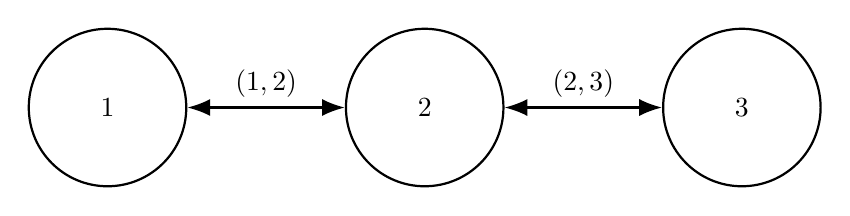
\begin{tikzpicture}[{Latex[scale=1.25]}-{Latex[scale=1.25]}, thick]
			% Grids
			\node[main node] (1) {$1$};
			\node[main node] [right = 2cm of 1] (2) {$2$};
			\node[main node] [right = 2cm of 2] (3) {$3$};
			% Paths
			\path[draw,thick]
			(1) edge node [above] {$(1, 2)$} (2)
			(2) edge node [above] {$(2, 3)$} (3);
		\end{tikzpicture}
	}
\end{minipage} \hfill
\begin{minipage}{0.35\textwidth}
	\begin{equation*}
		\matr{A} = \begin{pmatrix}
			0   & 1  & 0 \\
			- 1 & 0  & 1 \\
			0   & -1 & 0
		\end{pmatrix}
	\end{equation*}
\end{minipage}
\vspace{0.5cm}


and the associated line graph is,

\vspace{0.5cm}
\begin{minipage}{0.6\textwidth}
	\resizebox{0.7\textwidth}{!}{
		\begin{tikzpicture}[{Latex[scale=1.25]}-{Latex[scale=1.25]}, thick]
			% Grids
			\node[main node] (12) {$(1, 2)$};
			\node[main node] [right = 2cm of 1] (23) {$(2, 3)$};
			% Paths
			\path[draw,thick]
			(12) edge node [above] {$2$} (23);
		\end{tikzpicture}
	}
\end{minipage} \hfill
\begin{minipage}{0.35\textwidth}
	\begin{equation*}
		\matr{G} = \begin{pmatrix}
			0  & 1 \\
			-1 & 0
		\end{pmatrix}
	\end{equation*}
\end{minipage}
\vspace{0.5cm}


The Nash bargaining solution is then,

\begin{equation*}
	\begin{split}
		\begin{pmatrix}
			P^{(1, 2)} \\
			P^{(2, 3)}
		\end{pmatrix} &= (2\matr{I} + \matr{G})^{-1} \begin{pmatrix}
			(\Delta X / Y)^{(1, 2)} \\
			(\Delta X / Y)^{(2, 3)}
		\end{pmatrix} \\
		&= \begin{pmatrix}
			2  & 1 \\
			-1 & 2
		\end{pmatrix}^{-1} (\Delta X \oslash Y)\\
		&= \frac{1}{2 \cdot 2 - 1 \cdot (-1)} \begin{pmatrix}
			2 & - 1 \\
			1 & 2
		\end{pmatrix} (\Delta X \oslash Y) \\
		&= \frac{1}{5} \begin{pmatrix}
			2 & - 1 \\
			1 & 2
		\end{pmatrix} (\Delta X \oslash Y)
	\end{split}
\end{equation*}

In Appendix \ref{a:three_firms} I derive the matrix $(2 \matr{I} + \matr{G})^{-1}$ as a Neumann series.

Using then Equation (\ref{foc_grid}),

\begin{equation}
	\begin{split}
		P + \partial P \circ Y &= \left[ (2 \matr{I} + \matr{G})^{-1} - \diag(2 \matr{I} + \matr{G})^{-1}  \right] (\Delta X \oslash Y) \\
		&= \frac{1}{5} \left[ \begin{pmatrix}
				2 & - 1 \\
				1 & 2
			\end{pmatrix} -  \begin{pmatrix}
				2 & 0 \\
				0 & 2
			\end{pmatrix}\right] (\Delta X \oslash Y) \\
		&= -\frac{1}{5} \matr{G} (\Delta X \oslash Y)
	\end{split}
\end{equation}

Leveraging the fact that 3 and 1 have only one neighbor to trade with, $N(3) = N(1) = \set{2}$, in equilibrium their demand needs to equal the trade with 2. Namely,

\begin{equation}
	X_3 = Y^{2, 3} \text{ and } X_1 = Y^{1, 2}
\end{equation}

hence,

\begin{equation}
	\begin{split}
		\Delta X \oslash Y &= \begin{pmatrix}
			\frac{X_1 \cdot p_1 - X_2 \cdot p_2}{X_1} &
			\frac{X_2 \cdot p_1 - X_3 \cdot p_2}{X_3}
		\end{pmatrix}^{T} \\
		&= \begin{pmatrix}
			p_1 - \frac{X_2}{X_1} \cdot p_2 &
			\frac{X_2}{X_3} \cdot p_2 - p_3
		\end{pmatrix}^{T}
	\end{split}
\end{equation}

Using this we can rewrite

\begin{equation}
	P + \partial P \circ Y = - \frac{1}{5} \matr{G} \begin{pmatrix}
		p_1 - \frac{X_2}{X_1} \cdot p_2 \\
		\frac{X_2}{X_3} \cdot p_2 - p_3
	\end{pmatrix} = \frac{1}{5} \begin{pmatrix}
		p_3 - \frac{X_2}{X_3} \cdot p_2 \\
		p_1 - \frac{X_2}{X_1} \cdot p_2
	\end{pmatrix}
\end{equation}

The firms' three first order condition now be used to find $X_1, X_2, X_3$,

\begin{alignat*}{3}
	p_2 + \frac{X_2}{\partial X_2 / p_2} &  & = \frac{1}{5} \left( p_3 - \frac{X_2}{X_3} \cdot p_2  \right) &  & = p_1 + \frac{X_1}{\partial X_1 / p_1} \\
	p_2 + \frac{X_2}{\partial X_2 / p_2} &  & = \frac{1}{5} \left( p_1 - \frac{X_2}{X_1} \cdot p_2  \right) &  & = p_3 + \frac{X_3}{\partial X_3 / p_3}
\end{alignat*}

In order to simplify, let,

\begin{equation}
	F_i := p_i +  \frac{X_i}{\partial X_i / p_i}
\end{equation}

The condition implies,

\begin{equation}
	F_1 = F_2 = F_3 = \frac{p_1}{5} + \left(- \frac{X_2 \cdot p_2}{5} \right) \cdot \frac{1}{X_1} = \frac{p_3}{5} + \left(- \frac{X_2 \cdot p_2}{5} \right) \cdot \frac{1}{X_3}
\end{equation}

We can use this equation to eliminate any dependence on $p_2$,

\begin{equation}
	\begin{split}
		\frac{p_1}{5} + \left(- \frac{X_2 \cdot p_2}{5} \right) \cdot \frac{1}{X_1} &= F_3 \\
		- \frac{X_2 \cdot p_2}{5} &= \left( F_3 - \frac{p_1}{5} \right) \cdot X_1
	\end{split}
\end{equation}

which implies

\begin{equation}
	\begin{split}
		\frac{p_3}{5} + \left(- \frac{X_2 \cdot p_2}{5} \right) \cdot \frac{1}{X_3} &= F_1 \\
		\frac{p_3}{5} + \left( F_3 - \frac{p_1}{5} \right) \cdot \frac{X_1}{X_3} &= F_1 \\
		\frac{1}{5} \cdot (p_3 - p_1) + \frac{X_1}{X_3} \cdot F_3 - F_1 &= 0
	\end{split}
\end{equation}

In equilibrium, $F_3 = F_1$, hence, writing the explicit dependence on $p_i$,

\begin{equation}
	\frac{1}{5} \cdot (p_3 - p_1) + \left( \frac{X_1(p_1)}{X_3(p_3)} - 1 \right) \cdot F_1(p_1)= 0
\end{equation}

\newpage
\subsection{Bottleneck}


\vspace{0.5cm}

\begin{center}
	\resizebox{0.8\textwidth}{!}{
		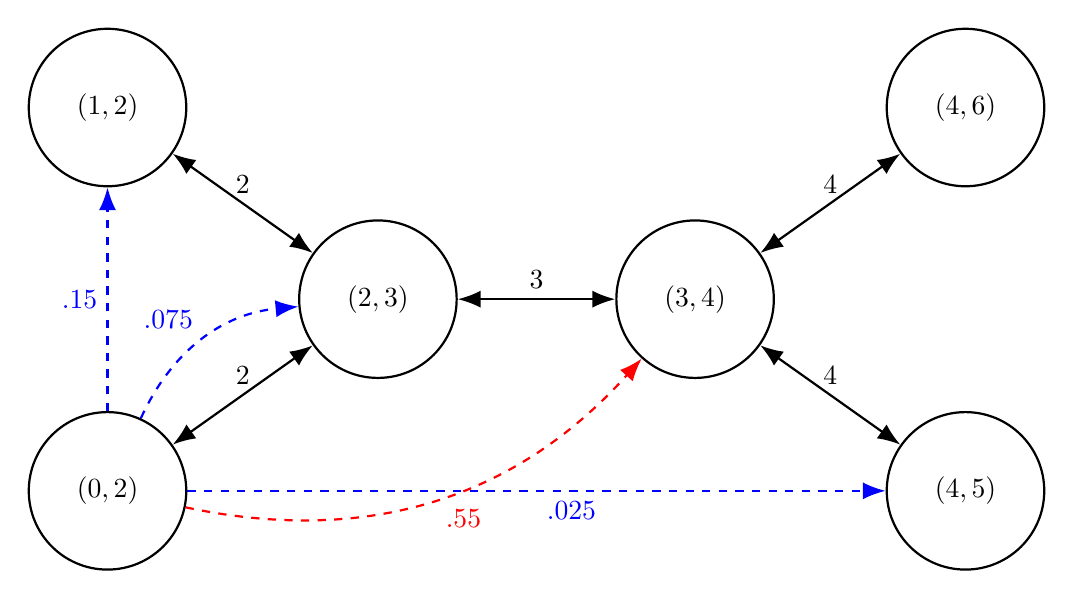
\begin{tikzpicture}[{Latex[scale=1.25]}-{Latex[scale=1.25]}, thick]
			% Grids
			\node[main node] (23) {$(2, 3)$};
			\node[main node] [below left = 1cm and 2cm of 23] (02) {$(0, 2)$};
			\node[main node] [above left = 1cm and 2cm of 23] (12) {$(1, 2)$};
			\node[main node] [right = 2cm of 23] (34) {$(3, 4)$};
			\node[main node] [below right = 1cm and 2cm of 34] (45) {$(4, 5)$};
			\node[main node] [above right = 1cm and 2cm of 34] (46) {$(4, 6)$};

			% Paths
			\path[draw,thick]
			(02) edge node [above] {$2$} (23)
			(12) edge node [above] {$2$} (23)
			(23) edge node [above] {$3$} (34)
			(45) edge node [above] {$4$} (34)
			(46) edge node [above] {$4$} (34);

			% Weights
			\path[draw, thick, dashed, -{Latex[scale=1.25]}]
			(02) edge [color=blue] node [left] {$.15$} (12)
			(02) edge [bend left, color=blue] node [above left] {$.075$} (23)
			(02) edge [bend right, color=red] node [below right] {$.55$} (34)
			(02) edge [color=blue] node [below right] {$.025$} (45);
		\end{tikzpicture}
	}
\end{center}
\begin{equation*}
	(\matr{2I - G})^{-1} = \begin{pmatrix}
		0.425  & -0.15 & -0.075 & 0.05 & -0.025 & -0.025 \\
		0.15   & 0.3   & 0.15   & -0.1 & 0.05   & 0.05   \\
		-0.075 & -0.15 & 0.425  & 0.05 & -0.025 & -0.025 \\
		0.05   & 0.1   & 0.05   & 0.3  & -0.15  & -0.15  \\
		0.025  & 0.05  & 0.025  & 0.15 & 0.425  & -0.075 \\
		0.025  & 0.05  & 0.025  & 0.15 & -0.075 & 0.425  \\
	\end{pmatrix}
\end{equation*}
\vspace{0.5cm}



\newpage
\subsection{Alternative path}

Consider now the more complex example,

\vspace{0.5cm}
\resizebox{\textwidth}{!}{
	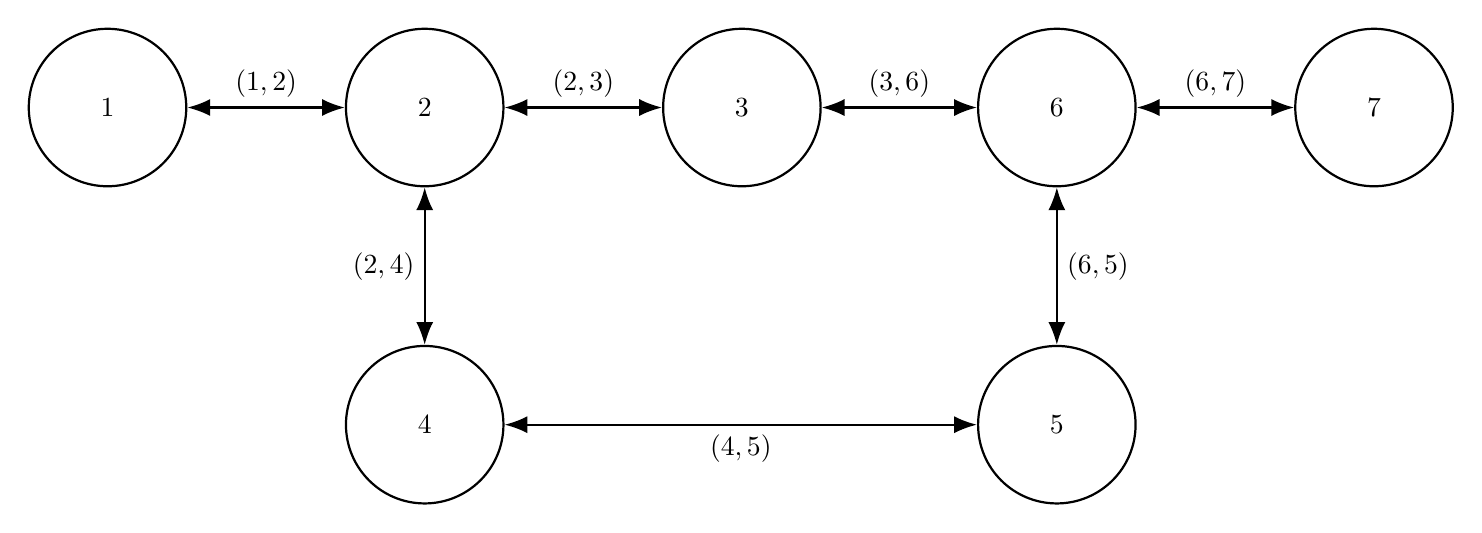
\begin{tikzpicture}[{Latex[scale=1.25]}-{Latex[scale=1.25]}, thick]
		% Grids
		\node[main node] (1) {$1$};
		\node[main node] [right = 2cm of 1] (2) {$2$};
		\node[main node] [right = 2cm of 2] (3) {$3$};
		\node[main node] [below = 2cm of 2] (4) {$4$};
		\node[main node] [right = 6cm of 2] (6) {$6$};
		\node[main node] [below = 2cm of 6] (5) {$5$};
		\node[main node] [right = 2cm of 6] (7) {$7$};
		% Paths
		\path[draw,thick]
		(1) edge node [above] {$(1, 2)$} (2)
		(2) edge node [above] {$(2, 3)$} (3)
		(3) edge node [above] {$(3, 6)$} (6)
		(2) edge node [left] {$(2, 4)$} (4)
		(4) edge node [below] {$(4, 5)$} (5)
		(6) edge node [right] {$(6, 5)$} (5)
		(6) edge node [above] {$(6, 7)$} (7);
	\end{tikzpicture}
}

\begin{equation*}
	\matr{A} = \begin{pmatrix}
		0  & 1  & 0  & 0  & 0  & 0  & 0 \\
		-1 & 0  & 1  & 1  & 0  & 0  & 0 \\
		0  & -1 & 0  & 0  & 0  & 1  & 0 \\
		0  & -1 & 0  & 0  & 1  & 0  & 0 \\
		0  & 0  & 0  & -1 & 0  & 1  & 0 \\
		0  & 0  & -1 & 0  & -1 & 0  & 1 \\
		0  & 0  & 0  & 0  & 0  & -1 & 0
	\end{pmatrix}
\end{equation*}

The associated link graph is,

\vspace{0.5cm}
\begin{minipage}{0.6\textwidth}
	\resizebox{\textwidth}{!}{
		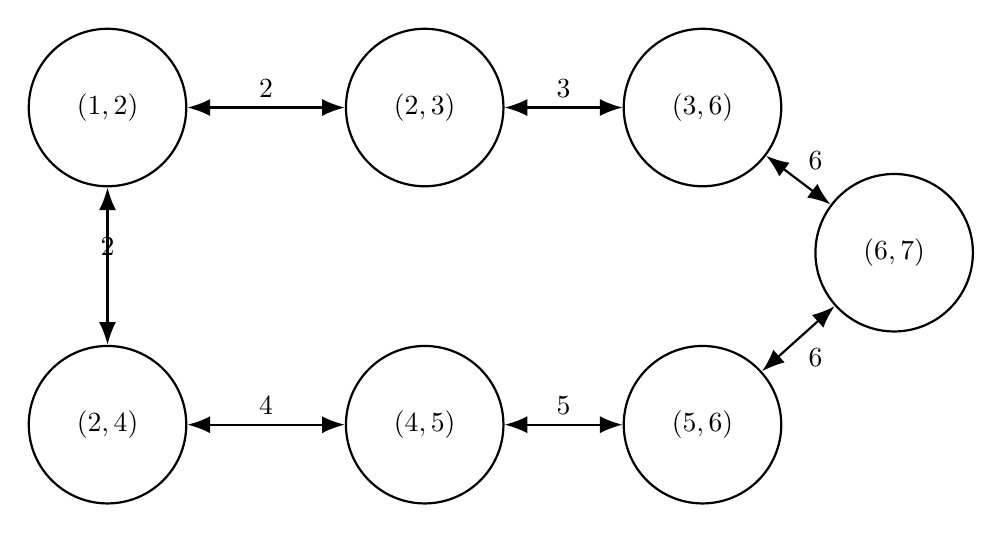
\begin{tikzpicture}[{Latex[scale=1.25]}-{Latex[scale=1.25]}, thick]
			% Grids
			\node[main node] (12) {$(1, 2)$};
			\node[main node] [right = 2cm of 12] (23) {$(2, 3)$};
			\node[main node] [right = 1.5cm of 23] (36) {$(3, 6)$};
			\node[main node] [below = 2cm of 12] (24) {$(2, 4)$};
			\node[main node] [right = 2cm of 24] (45) {$(4, 5)$};
			\node[main node] [right = 1.5cm of 45] (56) {$(5, 6)$};
			\node[main node] [above right = 0.75cm and 1cm of 56] (67) {$(6, 7)$};
			% Paths
			\path[draw,thick]
			(12) edge node [above] {$2$} (23)
			(12) edge node [above] {$2$} (24)
			(45) edge node [above] {$4$} (24)
			(56) edge node [above] {$5$} (45)
			(23) edge node [above] {$3$} (36)
			(36) edge node [above right] {$6$} (67)
			(56) edge node [below right] {$6$} (67);
		\end{tikzpicture}
	}
\end{minipage} \hfill
\begin{minipage}{0.35\textwidth}

	\begin{equation*}
		\matr{G}(\matr{A}) = \begin{pmatrix}
			0  & 1  & 1  & 0  & 0  & 0 & 0  \\
			-1 & 0  & 0  & 1  & 0  & 0 & 0  \\
			-1 & 0  & 0  & 0  & 1  & 0 & 0  \\
			0  & -1 & 0  & 0  & 0  & 1 & 0  \\
			0  & 0  & -1 & 0  & 0  & 0 & 1  \\
			0  & 0  & 0  & -1 & 0  & 0 & -1 \\
			0  & 0  & 0  & 0  & -1 & 1 & 0
		\end{pmatrix}
	\end{equation*}
\end{minipage}

\vspace{1em}
which yields,

\begin{equation*}
	(2\matr{I} + \matr{G})^{-1} = 0.354 \cdot \matr{I} + \begin{pmatrix}
		0     & -0.144 & -0.149 & 0.065  & 0.056  & -0.015 & -0.036 \\
		0.149 & 0      & -0.056 & -0.144 & 0.036  & 0.065  & 0.015  \\
		0.144 & -0.065 & 0      & 0.015  & -0.149 & -0.036 & 0.056  \\
		0.056 & 0.149  & -0.036 & 0      & -0.015 & -0.144 & -0.065 \\
		0.065 & -0.015 & 0.144  & 0.036  & 0      & 0.056  & -0.149 \\
		0.036 & 0.056  & 0.015  & 0.149  & 0.065  & 0      & 0.144  \\
		0.015 & -0.036 & 0.065  & -0.056 & 0.144  & -0.149 & 0      \\
	\end{pmatrix}
\end{equation*}

% ------------------------

\iffalse % Weighted case

	\section{Weighted one prosumer case}

	Assume the local market has a one prosumers with type indicator $\mathbf{1}\{h_t = f\} = \eta_t$.

	\begin{equation}
		\begin{split}
			X_t(p) &= \eta_t \cdot x_{t, f} + (1 - \eta_t) \cdot x_{t, c} \\
			&= \eta_t \cdot \frac{m_t - g_f(m_t, p)}{p} + (1 - \eta_t) \cdot \frac{m_t - g_c(m_t, p)}{p}
		\end{split}
	\end{equation}


	Then,
	\begin{equation}
		\begin{split}
			\frac{\partial X}{\partial p} &= \frac{1}{p^2} \cdot \left[ \eta_t \cdot \left(\frac{\partial}{\partial p} g_f \cdot p + m_t - g_f \right) + (1 - \eta_t) \cdot \left(\frac{\partial}{\partial p} g_c \cdot p + m_t - g_c \right) \right] \\
			&=\frac{1}{p^2} \left[m_t + \eta_t \cdot \left( g^\prime_f \cdot p - g_f \right) + (1 - \eta_t) \cdot \left( g^\prime_c \cdot p - g_c \right) \right]
		\end{split}
	\end{equation}

	Hence,

	\begin{equation}
		\begin{split}
			\frac{X}{\partial X / \partial p} = p \cdot \frac{m_t - \eta_t \cdot g_f + (\eta_t - 1) \cdot g_c}{m_t + \eta_t \cdot ( g^\prime_f \cdot p - g_f ) + (1 - \eta_t) \cdot (g^\prime_c \cdot p - g_c)}
		\end{split}
	\end{equation}

	\begin{equation}
		\begin{split}
			\frac{X}{\partial X / \partial p} + p &= p \cdot \frac{m_t - \eta_t \cdot g_f + (\eta_t - 1) \cdot g_c}{m_t + \eta_t \cdot ( g^\prime_f \cdot p - g_f ) + (1 - \eta_t) \cdot (g^\prime_c \cdot p - g_c)} + 1 \\
			&= p \cdot  \frac{m_t - \eta_t \cdot g_f + (\eta_t - 1) \cdot g_c + m_t + \eta_t \cdot ( g^\prime_f \cdot p - g_f ) + (1 - \eta_t) \cdot (g^\prime_c \cdot p - g_c)}{m_t + \eta_t \cdot ( g^\prime_f \cdot p - g_f ) + (1 - \eta_t) \cdot (g^\prime_c \cdot p - g_c)} \\
			&= p \cdot \frac{2 \cdot m_t + \eta_t \cdot (g^\prime_f \cdot p - 2\cdot g_f) + (1 - \eta_t) \cdot (g^\prime_c \cdot p - 2\cdot g_c)}{m_t + \eta_t \cdot ( g^\prime_f \cdot p - g_f ) + (1 - \eta_t) \cdot (g^\prime_c \cdot p - g_c)}
		\end{split}
	\end{equation}

\fi

\iffalse % Case with discrete N
	Then,

	\begin{equation}
		\begin{split}
			X_t(p) &= \sum_{i\in f}  x_{t, i} + \sum_{j \in c} x_{t, j} \\
			&= \frac{\sum_{i \in f}  \left[m_{t, i} - g_f(m_{t, i}, p_t)\right]  + \sum_{j \in c}  \left[m_{t, j} - g_c(m_{t, j}, p_t)\right]}{p}
		\end{split}
	\end{equation}

	hence,

	\begin{equation}
		\begin{split}
			\frac{\partial}{\partial p} X_t(p) = &p \cdot \left[\sum_{i \in f} \frac{\partial}{\partial p} g_f + \sum_{j \in c} \frac{\partial}{\partial p} g_c  \right] + \\
			&+ \sum_{i \in f}  \left[m_{t, i} - g_f(m_{t, i}, p_t)\right]  + \sum_{j \in c}  \left[m_{t, j} - g_c(m_{t, j}, p_t)\right] = 0 \\
			0 &= \sum_{i \in f} \left[ m_{t, i} - g_f(m_{t, i}, p_t) + p \cdot \frac{\partial}{\partial p} g_f \right] + \sum_{j \in c}\left[m_{t, j} - g_c(m_{t, j}, p_t) +  p \cdot\frac{\partial}{\partial p} g_c\right]
		\end{split}
	\end{equation}

\fi
\newpage
\section{Figures}

\begin{figure}[!ht]
	\centering
	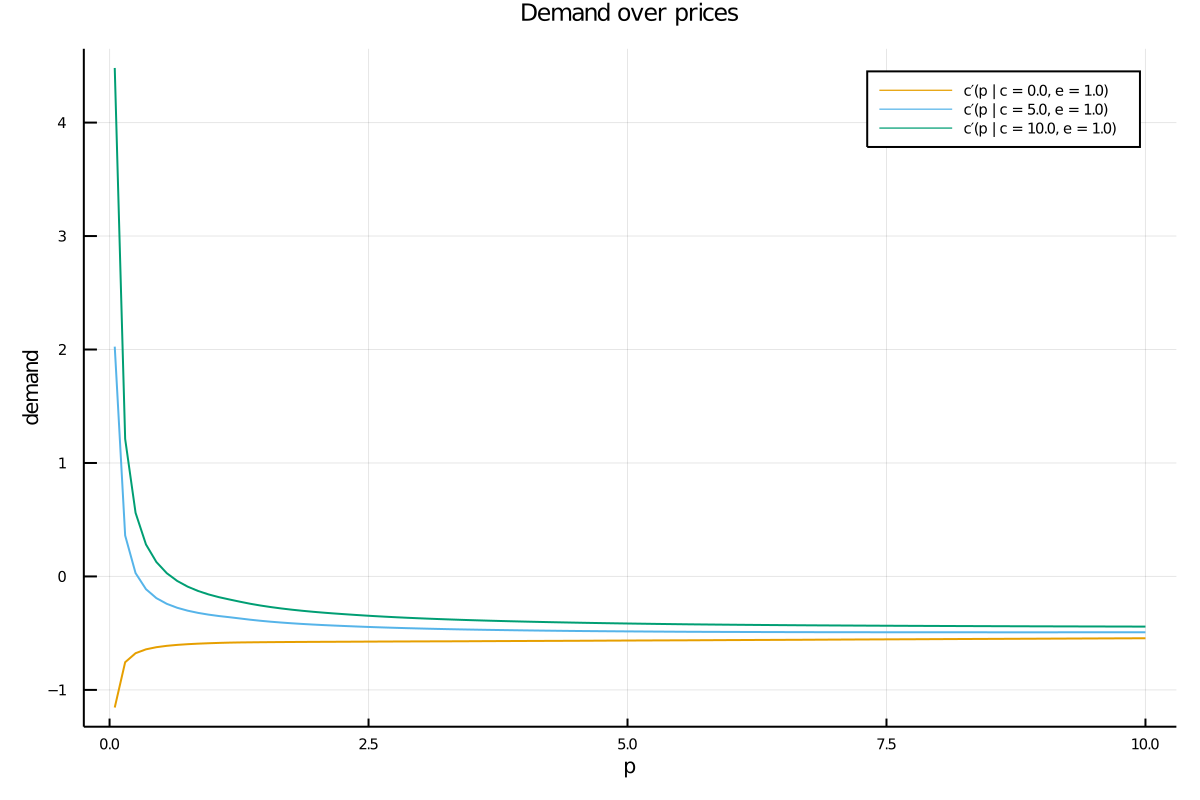
\includegraphics[width=0.9\textwidth]{../../plots/markets/pricedemand.png}
	\caption{Electricity demand curve for an agent}
	\label{fig:demand}
\end{figure}

\begin{figure}[!ht]
	\centering
	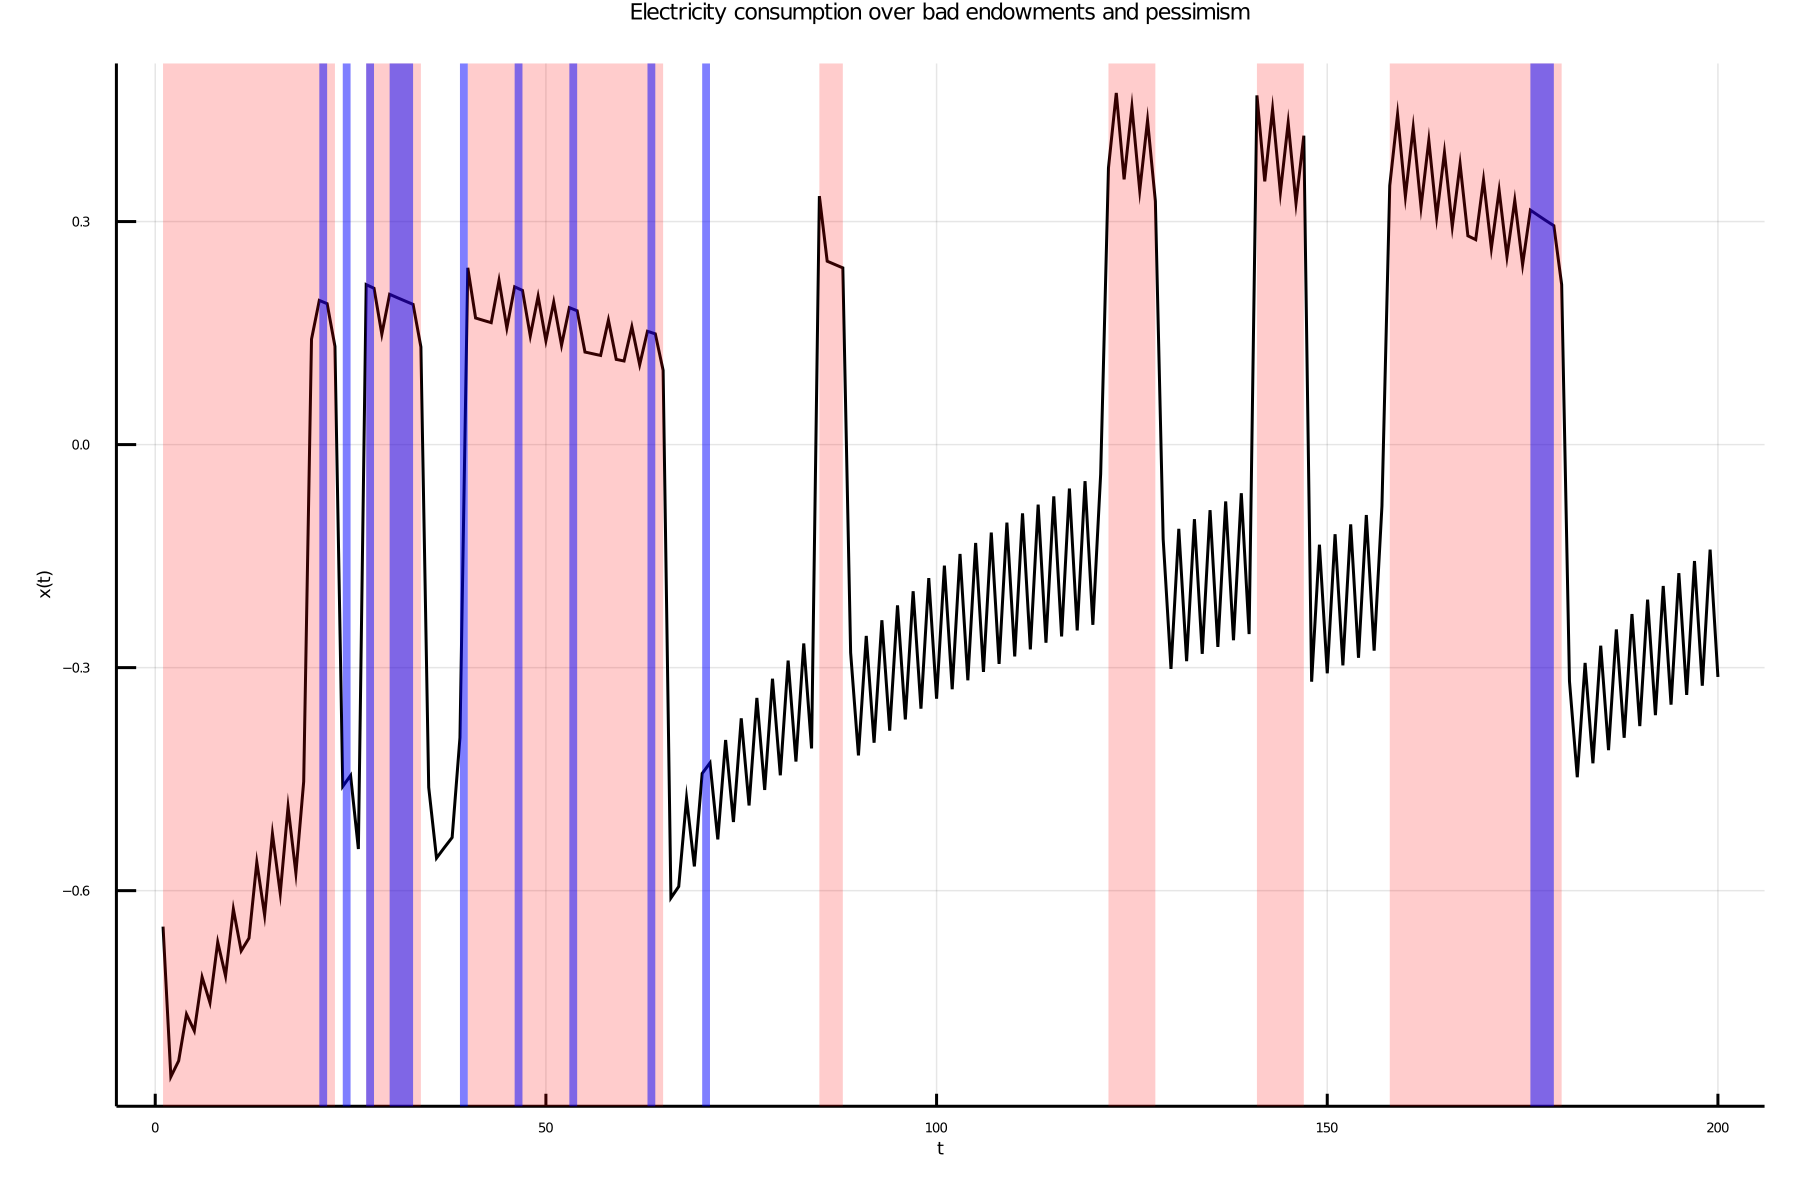
\includegraphics[width=0.9\textwidth]{../../plots/markets/simul.png}
	\caption{Simulation of an agent with switching forecasting rule and $AR(1)$ price process}
	\label{fig:sim}
\end{figure}

\begin{figure}[!ht]
	\centering
	\includegraphics[width=0.9\textwidth]{../../plots/markets/kde.png}
	\caption{Prices in the above simulation}
	\label{fig:price}
\end{figure}


\newpage
\appendix

\section{Epstein-Zin preferences}


A better formulation, using Epstein-Zin preferences,

\begin{equation}
	U_t = \left[ (1 - \beta) \cdot u(x_t)^{\frac{\phi - 1}{\phi}} + \beta \cdot \mu_t(U_{t+1})^{\frac{\phi - 1}{\phi}} \right]^{\frac{\phi}{\phi - 1}}
\end{equation}

where the certainty equivalent is,

\begin{equation}
	\mu_t(U) = \E_t\left[ U^{1 - \gamma} \right]^{\frac{1}{1 - \gamma}}.
\end{equation}

As Caldara, introduce,

\begin{equation}
	\theta := \frac{1 - \gamma}{1 - \frac{1}{\phi}}.
\end{equation}


\section{Notes on $(2\matr{I} + \matr{G})^{-1}$} \label{a:inv}
\newcommand*{\G}{\matr{G}}
\newcommand*{\I}{\matr{I}}
\newcommand*{\B}{\matr{B}}


\subsection{Using Neumann series} \label{a:neumann}

The matrix $-\frac{1}{2}\G$ has $2$-norm smaller than $1$, hence the inverse is defined and is equal to the Neumann series,

\begin{equation}
	\left(\I + \frac{1}{2} \G\right)^{-1} = \sum^{\infty}_{k = 0} \left(-\frac{1}{2} \G\right)^k
\end{equation}

We can therefore rewrite,

\begin{equation}
	\begin{split}
		(2\I + \G)^{-1} &= \frac{1}{2}\left(\I + \frac{1}{2}\G\right)^{-1} \\
		&= \frac{1}{2} \sum^{\infty}_{k = 0} \left(-\frac{1}{2} \G\right)^k \\
		&= \sum^{\infty}_{k = 0} \frac{(-1)^k}{2^{k+1}} \G^k
	\end{split}
\end{equation}

\subsection{Three firms case} \label{a:three_firms}

If $\G = \begin{pmatrix}
		0 & 1 \\ -1 & 0
	\end{pmatrix}$, then $\G^k$ oscillates as follows,

\begin{center}
	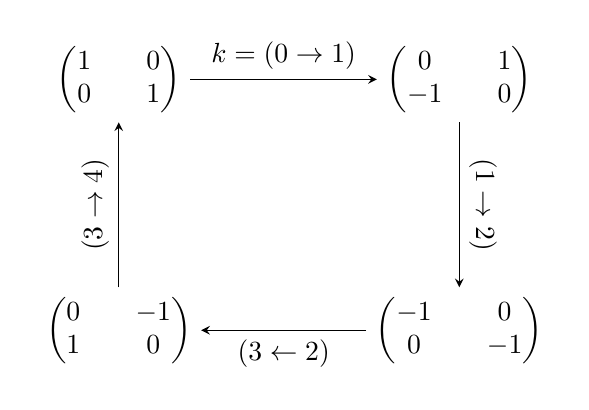
\begin{tikzpicture}
		\matrix (m) [matrix of math nodes,row sep=6em,column sep=6em,minimum width=2em]
		{
			\begin{pmatrix}
				1 & 0 \\ 0 & 1
			\end{pmatrix} & \begin{pmatrix}
				0 & 1 \\ -1 & 0
			\end{pmatrix} \\ \begin{pmatrix}
				0 & -1 \\ 1 & 0
			\end{pmatrix} &
			\begin{pmatrix}
				-1 & 0 \\ 0 & -1
			\end{pmatrix}  \\};
		\path[-stealth]
		(m-1-1) edge node [above] {$k = (0 \to 1)$} (m-1-2)
		(m-1-2) edge node [above, rotate=270] {$(1 \to 2)$} (m-2-2)
		(m-2-2) edge node [below] {$(3 \gets 2)$} (m-2-1)
		(m-2-1) edge node [above, rotate=90] {$(3 \to 4)$} (m-1-1);
	\end{tikzpicture}
\end{center}

hence we can rewrite,

\begin{equation}
	\begin{split}
		\sum^{\infty}_{k = 0} \frac{(-1)^k}{2^{k+1}} \G^k &= \frac{1}{2} \cdot \begin{pmatrix}
			1 & 0 \\ 0 & 1
		\end{pmatrix} - \frac{1}{4} \cdot \begin{pmatrix}
			0 & -1 \\ 1 & 0
		\end{pmatrix} + \frac{1}{8} \cdot \begin{pmatrix}
			-1 & 0 \\ 0 & -1
		\end{pmatrix} - \frac{1}{16} \begin{pmatrix}
			0 & -1 \\ 1 & 0
		\end{pmatrix} \ldots
	\end{split}
\end{equation}

The diagonal entry in this case yield the series,

\begin{equation}
	\begin{split}
		\left(\sum^{\infty}_{k = 0} \frac{(-1)^k}{2^{k+1}} \G^k\right)_{i, i} &= \frac{1}{2} - \frac{1}{8} + \frac{1}{32} - \frac{1}{128}... \\
		&= \frac{1}{2} \sum^\infty_{k = 0} \frac{(-1)^k}{4^k} = \frac{2}{5}
	\end{split}
\end{equation}

\subsection{Interpretation of $\G^k$}

Using the property, $\G_{i, j} = - \G_{j, i}$ we can rewrite every entry of the diagonal of $\G^k$,

\begin{equation}
	\begin{split}
		\G^2_{i, i} &= \sum^n_{m = 1} g_{i, m} \cdot g_{m, i} = - \sum^n_{m=1} g^2_{i, m} = - \deg(i) \\
		G^3_{i, i} &= \sum^n_{m=1} \G^2_{i, m} \cdot g_{m, i} = - \sum^n_{m=1} \deg(i) \cdot g_{m, i} = 0
	\end{split}
\end{equation}

\textbf{To do: The tendency continues and has to do with the binomial formula and the number of cycle in the link graph}

\subsection{Other properties}

Using Woodbury matrix identity, we know that,

\begin{equation}
	\begin{split}
		(2\I + \G)^{-1} &= \frac{1}{2}\left(\I + \frac{1}{2}\G \right)^{-1} \\
		&= \frac{1}{2} \left( \I - \frac{1}{2}\G \left(\I +\frac{1}{2}\G\right)^{-1} \right)
	\end{split}
\end{equation}


Note that $\Tr{\left(\I + \frac{1}{2}\G \right)} = n$.

Furthermore, since, $p_{(-\G)}(x) = \det{(x \I - \G)}$, we are interested in $p_{(-\G)}(2)$.

\iffalse
	\section{Jacobian of $P$}

	Let $g(x) = (2\matr{I} + \matr{G})^{-1} x = \B x$ and $f(x) = \Delta X \oslash x$. Then $P = (g \circ f)(Y)$.

	By the chain rule,

	\begin{equation}
		J_P(Y) = (J_f \circ g)(Y) \cdot J_g(Y)
	\end{equation}

	Here,

	\begin{equation}
		\begin{split}
			J_f(x) &= \diag\left( - \Delta X \oslash x^{\circ 2} \right) \\
			J_g(x) &= \B.
		\end{split}
	\end{equation}

	For example, $J_P$ evaluated at $a = \begin{pmatrix}
			a_1 & a_2 & a_3
		\end{pmatrix}^T$ is,

	\begin{equation}
		J_P(a) = - \B \begin{pmatrix}
			\Delta X_1 / a_1^2 & 0                  & 0                  \\
			0                  & \Delta X_2 / a_2^2 & 0                  \\
			0                  & 0                  & \Delta X_3 / a_3^2
		\end{pmatrix} \B a
	\end{equation}

\fi


\end{document}